We will now describe the kernel implementation.

\subsection{Kernel writing}
The kernel in itself is written in CUDA in the GASAL2 library. It should exactly replicate the behaviour of the original function in BWA-MEM, called \verb|ksw_extend|. In the remainder of the thesis we will refer to the original function with its name, \verb|ksw_extend|, and to its GPU implementation as the \verb|ksw_kernel|.

We have seen before that previous kernels in GASAL2 were written as C++ template functions. It has been considered using the existing local alignment kernel template to derive an alternate kernel with the starting scores. This could have reduced the amount of code to maintain. However, there are many differences between the seed-only kernel and the local kernel. In particular, an important number of speed-up techniques are present in \verb|ksw_extend| and the code written to implement them presented many differences with the way the local kernel is written. Therefore, we implement a new kernel that follows the seed-only paradigm.

The kernel is built by copying the original \verb|ksw_extend| and renaming the variables to follow naming convention used in GASAL2 kernels. Initially, to test the implementation, we follow the loop structure used in \verb|ksw_extend| in which the fact that data is compressed is not exploited. The behaviour is simply to fetch the current base from query and target and calculate the cell of the dynamic programming matrix. Therefore, the pseudocode is the same as presented previously in Algorithm~\ref{algo:local} in Subsection~\ref{sec:local}.

We introduce the use of compressed data by fetching the 8 bases in the 32-bit words from query and target. This adds two innermost loops in the algorithm to perform the alignment tile by tile, using square tiles of $8 \times 8 = 64$ bases.

Because of memory constraints, the whole matrix is not stored in memory. Since only the north, west, and north-west cells are needed for the computation, only one full row having the length of the query string and a column of 8 cells need to be stored. These are shown in Figure~\ref{fig:visualisation-aid-tile}. All cells are computed in the order given by their number. When a full column is computed, the orange column moves one step on the right, taking the place of the cells numbered 1 to 8; then when cells 9 to 16 are computed, the orange column moves forward to take their place, and so on. This column is the western cells used to compute the score. When all cells in the tile are computed, the 8-cell section of the yellow row moves 8 cells south, taking the place of the cells numbered 8, 16, 24 ... 64. When the cyan tile is computed, the royal blue one is computed, then the navy blue, then the next line.

\begin{figure}[h!]
	\centering
	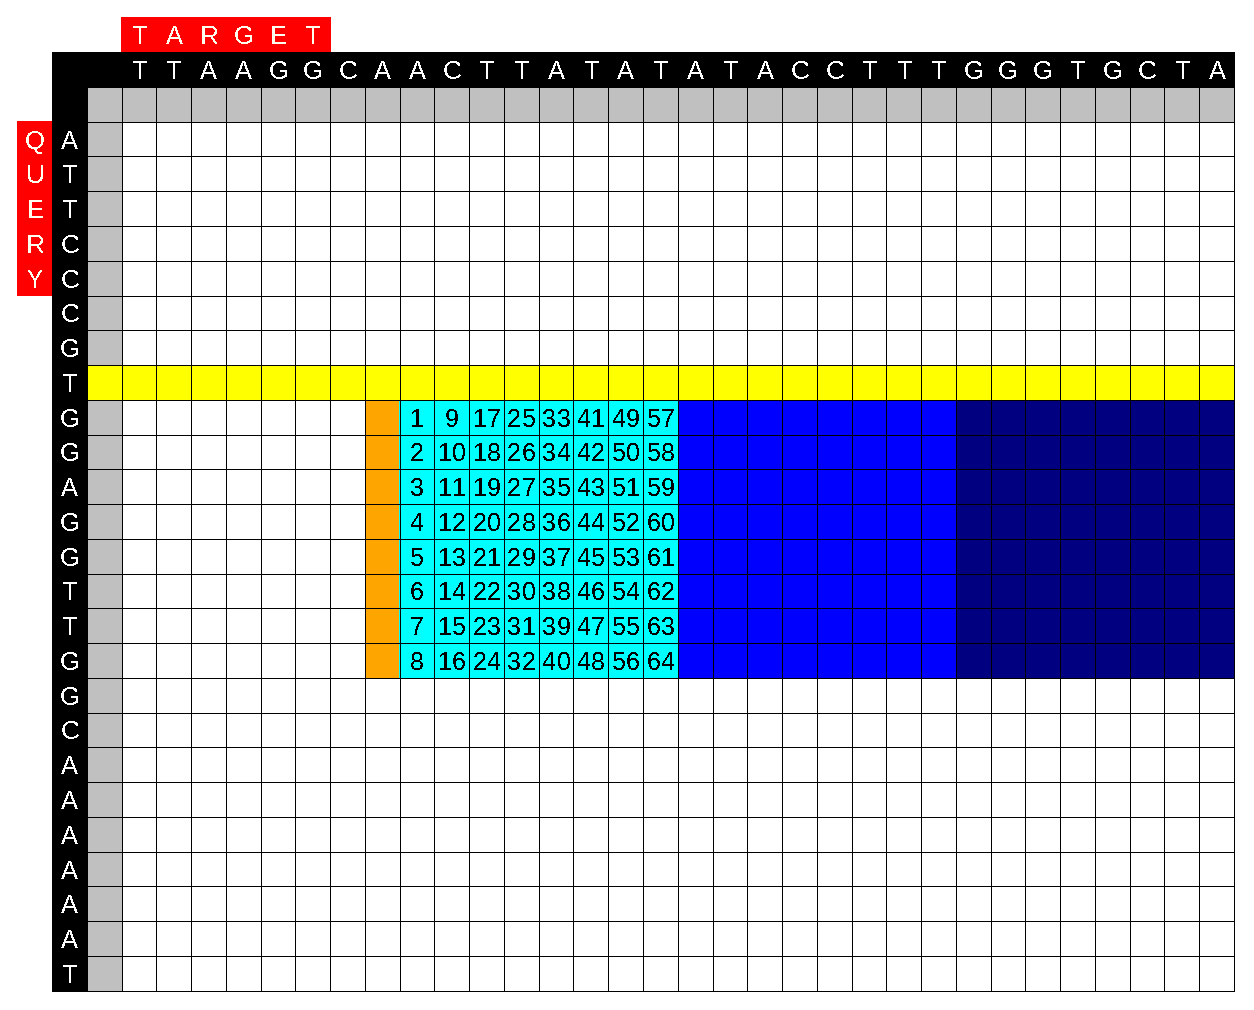
\includegraphics[width=0.9\linewidth]{visualisation-aid-tile}
	\caption{Visualisation of the tile-based matrix computation. Only the yellow row and the orange column are stored in memory.}
	\label{fig:visualisation-aid-tile}
\end{figure}

%The algorithm changes as reported in paper ~\cite{Ahmed:gasal}.

Finally, we introduce again some computing optimisations that we initially disabled, in particular, z-dropoff. This optimisation allows to skip the calculation of some cells of the matrix provided the score drops below a certain threshold. When this happens, it usually means that the alignment will not improve because the difference between the two sequences grew too big, so it is usually better to stop computing altogether instead of wasting time trying to align two sequences that are very different.

With all of this implemented, the pseudocode for the kernel is shown in Algorithm~\ref{algo:kernel}. Some parts detailed in Algorithm~\ref{algo:local} are only summarised here for readability.
\begin{algorithm}[h!]
	\caption{ksw$\_$kernel algorithm}
	\label{algo:kernel}
	\begin{algorithmic}[1] % The number tells where the line numbering should start
		\Procedure{Seed-extension kernel}{$query\_string$, $target\_string$, $query\_length$, $target\_length$, $initial\_score$, $zdrop$} \Comment{$TILE\_SIDE = 8$}
		
		
		\State Initialise score
		\State Initialise maximum score $score \leftarrow 0$ and maximum positions $(max\_query, max\_target) \leftarrow (0, 0)$
		%\State Initialise global maximum score $gscore \leftarrow 0$ and global maximum positions $(gmax\_query, gmax\_target) \leftarrow (0, 0)$
		%\For{i from -1 to $query\_length$}
		%\State $S_{i, -1} \leftarrow 0$
		%\EndFor	
		
		%\For{j from -1 to $target\_length$}
		%\State $S_{-1, j} \leftarrow 0$	
		%\EndFor
		\State $query\_batch\_regs \leftarrow query\_length / TILE\_SIDE + 1$
		\State $target\_batch\_regs \leftarrow target\_length / TILE\_SIDE + 1$
		
		%\State \emph{compute S matrix}
		\For {$target\_tile\_id$ from $0$ to $(target\_batch\_regs-1)$}
		\State $gpac \leftarrow$ Fetch a pack of 8 bases from $target\_string$ at position $target\_tile\_id$ (int32)
		
		\For {$target\_base\_id$ from $0$ to $TILE\_SIDE-1$}
		\State $i = target\_tile\_id * TILE\_SIDE + target\_base_i$
		
		\State $target\_base_j \leftarrow $ read base in $gpac$ at position $target\_base\_id$ 
		\State Compute first column of the matrix
		
		\For {$query\_tile\_id$ from $0$ to $(query\_batch\_regs-1)$}
		\State $rpac \leftarrow$ Fetch a pack of 8 bases from $query\_string$ at position $query\_tile\_id$ (int32)
		
		\For {$query\_base\_id$ from $0$ to $TILE_SIDE-1$}
		\State $query\_base_j \leftarrow $ read base in $rpac$ at position $query\_base\_id$ 
		
		\State $j = query\_tile\_id * TILE\_SIDE + query\_base_j$
		
		\If{$i < beg$}
		\State continue
		\EndIf
		\If{$i >= end$}
		\State break
		\EndIf
		
		\State Compute $S[i,j]$, $G_{A}[i,j]$ and $G_{B}[i,j]$
		
		% S = H (dans le C), G_A = E (dans le C), G_B = F (dans le C)
		
		\EndFor %query base
		\EndFor %query tile
		%% Zdrop
		\If{$j == query\_length$}
		\State Store global score and global end position
		\EndIf
		\If{maximum calculated score > previous maximum}
		\State Store new maximum score and new end position ($max\_query, max\_target$)
		\ElsIf{$zdrop > 0$}
		\If{the current score dropped more than $zdrop$ since the last maximum score}
		\State break
		\EndIf
		\EndIf
		
		%% cell-skipping
		\State Cell-skipping: $beg \leftarrow$ first cell of the stored row with non-zero score
		\State Cell-skipping: $end \leftarrow$ last cell of the stored row with non-zero score
		\EndFor %target base
		\EndFor %target tile
		
		\State Find $i_{max}$ and $j_{max}$ for which $S_{i_{max}, j_{max}} = max(S_{i,j})$
		\State $score \leftarrow S_{i_{max}, j_{max}}$
		\State $end\_position\_query \leftarrow i_{max}$
		\State $end\_position\_target \leftarrow j_{max}$
		
		\EndProcedure
		
	\end{algorithmic}
\end{algorithm}


\subsection{Score comparison}

To verify the correctness of this implementation, a modified version of BWA-MEM is made from the original BWA-MEM~\cite{lh3:bwa}. This version is hosted on GitHub~\cite{j-levy:bwa} and has different branches to switch from one behaviour to another, to compare the results with the GPU-accelerated implementation.

In a branch called \verb|seedonly-time|, we introduce our seed-only method instead of the original BLAST-like behaviour. As the name suggests, the time for each processing step is monitored and reported at the end of the program for each CPU thread.

The results are in the Sequence Alignment/Map (SAM) format, commonly used for DNA mapping. SAM is text-based, extensively documented~\cite{samtools:sam} and widespread among DNA-related programs. It is the default format output for BWA. Using \verb|diff|~\cite{misc:gnudiff} and other regular UNIX tools, we can compare the number of lines that differ between the reference program and a modified version. Knowing the original number of lines, we can derive a percentage of difference between the files, as shown on Listing~\ref{lst:diff}.

\begin{listing}[ht]
	\begin{minted}[
	fontsize=\footnotesize,
	linenos,
	breaklines,
	frame=single]{bash}
#!/bin/bash
DIFFLINES=$(diff --suppress-common-lines --speed-large-files -y $1 $2 | grep "[|><]" | wc -l)
TOTALLINES1=$(cat $1 | wc -l)
PERCENTDIFF=$(bc -l <<< "scale=2; (100*$DIFFLINES)/$TOTALLINES1")

echo "Different lines between " $1 " and " $2 " = " $DIFFLINES
echo "Total numer of lines in" $1 " = " $TOTALLINES1
echo "Difference = " $PERCENTDIFF "%"
	\end{minted}
	\caption{Bash script to show percentage of difference between two files}
	\label{lst:diff}
\end{listing}

